% ================================= preamble ===================================
% To compile this document on your own machine, run the following commands in
% the terminal:
%   pdflatex main
%   biber main
%   makeglossaries main
%   pdflatex main
%   pdflatex main
% In Overleaf, just click "Compile" once or CTRL-S.

% You can add options by entering text between the square brackets (`[]`).
%   Use the `noul` option if there is a conflict with the `\ul` command.
%   Use the `review` option when sending to committee members for review.
%   Use the `internal` option for a prospectus or graduate research paper.
%   Use the `style` option to customize citations: `style=ieee`.
\documentclass[]{afitthesis}

% ------------------------ Main document information ---------------------------

% NOTE: The following macros are the meta data of your document, like the title,
% author, and department. Some of these apply to the whole document. Some, like
% in the section after this, apply to the SF 298 form only. Several are
% commented out because they are probably not needed for your situation.

\title{Great Contribution to the Field of Things}
\author{John Smith}
% \authorsecond{} % Use these if other students contributed.
% \authorthird{}
% \authorfourth{}
\rank{First Lieutenant, USAF}
% \ranksecond{} % Use these if other students contributed.
% \rankthird{}
% \rankfourth{}
\previousdegrees{B.S.E.E.}
\newdegree{Master of Science in Electrical Engineering}
\graduationdate{March 2025} % expected month and year
\department{\ENG} % \ENY, \ENG, \ENP, \ENC, \ENS, or \ENV
% \doctype{dissertation} % Default is "thesis".
\docdesignator{AFIT-ENG-MS-XX-X-XXX} % provided by AFIT
% \address{} % Default is WPAFB.
% \disclaimer{} % Default distances the AF from the views of the paper.
% \copyrightstatement{} % Default claims ownership by US government.
\committee{ % rank name, Ph.D. \\ role
    {Albert Einstein, Ph.D.\\Chair},
    {Lt Col Michael Faraday, Ph.D.\\Member},
    {Maj Carl F. Gauss, M.S.\\Member}}
\abstract{Write your abstract here. This text should probably stay under 100
    words or so. Make sure to not put any personally-identifiable information
    about others in this text. This will be duplicated onto the SF-298 at the
    end of your thesis or dissertation. If it does not fit in the small box on
    the form, make a shorter version using the
    \texttt{\textbackslash{}sfAbstract} command.}
\keywords{earth; water; air; fire}
\dedication{To the one who loves me most.}
\acknowledgments{I would like to thank the entire committee for your great
    support.}

% Distribution and Control. Uncomment to specify.
% \cui{ % for Controlled Unclassified Information
%     Controlled By: AETC \\
%     Controlled By: AFIT/ENG \\
%     CUI Category(ies): PRVCY \\
%     Distribution: \DistB{CATEGORY}{DATE}{OFFICE} \\
%     POC: John Smith, 555-123-4567}
% \classified{ % for classified work
%     Classified By: \\
%     Derived From: \\
%     Declassify On: }
% \banner{cui} % automatically inserted into the header and footer

% -------------- SF 298 (Report Documentation Page) information ----------------

% Necessary fields
\sfStartDate{Sep 2023}
\sfEndDate{Mar 2024}
\sfContractNumber{XXXXXX-XX-X-XXXX}
\sfGrantNumber{}
\sfProgramElementNumber{}
\sfProjectNumber{XXXXXXXX}
\sfTaskNumber{}
\sfWorkUnitNumber{}
\sfSponsorAgency{AFXX/XXXX\\
    Building XXX, WPAFB OH 45433-7765\\
    DSN XXX-XXXX, COMM 937-XXX-XXXX, Email: first.last@us.af.mil }
\sfSponsorAcronyms{}
\sfSponsorReportNumber{}
\sfDistribution{\DistA}
\sfSupplementaryNotes{}
\sfReportClassification{}
\sfAbstractClassification{}
\sfPageClassification{}
\sfAbstractLimitation{UU}
\sfResponsiblePerson{Dr. Your Advisor, AFIT/ENG}
\sfPhoneNumber{(937) XXX-XXXX}
\sfClassification{}

% SF 298 Override default variables
% \sfReportDate{}       % defaults to today's date
% \sfReportType{}       % defaults to \doctype{}
% \sfTitle{}            % defaults to \title{}
% \sfAuthors{}          % defaults to \author{}, \rank{}
% \sfDepartment{}       % defaults to \department{}
% \sfAddress{}          % defaults to \address{}
% \sfDocDesignator{}    % defaults to \docdesignator{}
% \sfAbstract{}         % defaults to \abstract{}
% \sfSubjectTerms{}     % defaults to \keywords{}
% \sfPageCount{}        % defaults to total number of pages

% ------------------------- Glossaries and acronyms ----------------------------

% Example glossary and acronym definitions.
\newglossaryentry{latex}{name=\LaTeX{},
    description={Is a markup language specially suited
    for scientific documents}}
\newglossaryentry{maths}{name=mathematics,
    description={Mathematics is what mathematicians do}}
\newglossaryentry{formula}{name=formula,
    description={A mathematical expression}}
\newacronym{gcd}{GCD}{Greatest Common Divisor}
\newacronym{lcm}{LCM}{Least Common Multiple}

% ----------------------------- References files -------------------------------

% NOTE: Google "Overleaf Getting started with BibLaTeX" for guidance.
\addbibresource{refs.bib} % Name of the bibliography file
% The classification marking (e.g., "unclassified", "secret", etc.) can be
% specified for bibliographic entries in the `keywords` field in the bib file:
%    keywords = {unclassified},
% This will put the paragraphy marking (e.g., "(U)", "(S)", etc.) in front of
% the bibliographic entry.

% ------------------------------ Figures folder --------------------------------

% Define the default location to look for figures.
\graphicspath{{figures}}

% ============================== Body of paper =================================

\begin{document}
\maketitle % Creates all the prefatory pages.

\chapter{Introduction}

\emph{Contents of Chapter I, typically the introduction}

If you need help with writing \LaTeX{} code, refer to the GitLab project
\href{https://gitlab.com/davidwoodburn/latex-primer}{\LaTeX{} Primer} by David
Woodburn. Please also note the ``User Guide.pdf'' file included in this template.

The next page includes some example figures: Fig.~\ref{fig:hist} and
Fig.~\ref{fig:spec}.

Here is a citation: \textcite{savage2000} has some good information.

\begin{figure}
    \centering
    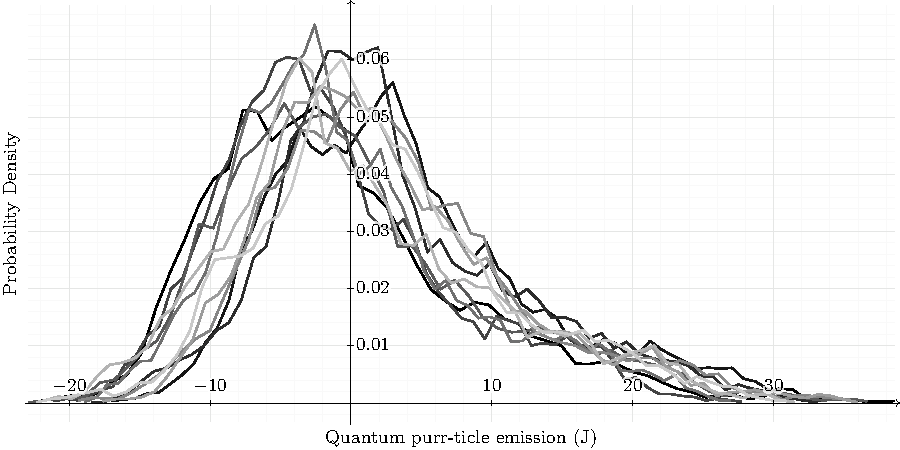
\includegraphics{fig_hist.pdf}
    \caption{Histogram of the emission energy for each of the data collects.}
    \label{fig:hist}
\end{figure}

\begin{figure}
    \centering
    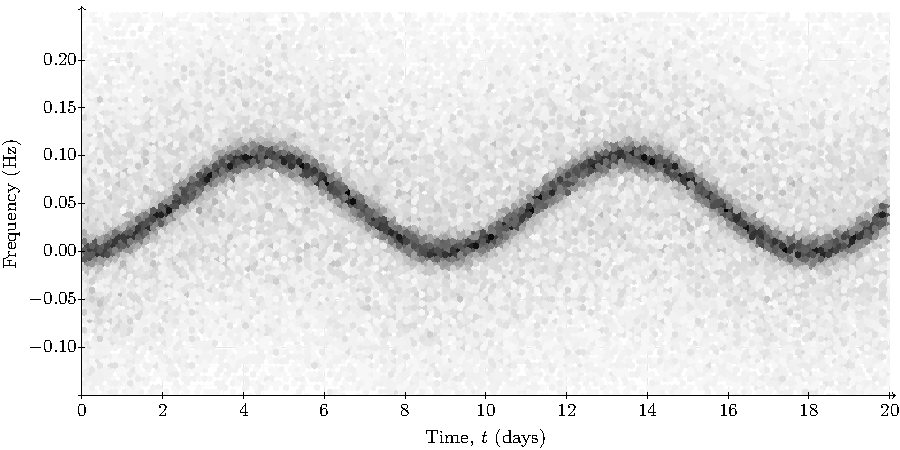
\includegraphics{fig_spec.pdf}
    \caption{Spectrogram of the emission energy over the 20-day period.}
    \label{fig:spec}
\end{figure}
\chapter{Literature Review}

\emph{Contents of Chapter II, typically includes background and literature
review}

\chapter{Methodology}

\emph{Contents of Chapter III, typically the methodology}

\chapter{Results and Analysis}

\emph{Contents of Chapter IV, typically the analysis}

\chapter{Conclusion}

\emph{Contents of Chapter V, typically the conclusion and future work}

\appendix % Necessary before any appendix chapters

\chapter{Acronyms}

This paragraph is an example of using the \verb|glossaries| package. The
\Gls{latex} typesetting markup language is especially suited for documents that
include \gls{maths}. \Glspl{formula} are rendered properly and easily, once one
gets used to the commands. Given a set of numbers, there are elementary methods
to compute its \acrlong{gcd}, which is abbreviated \acrshort{gcd}. This process
is similar to that used for the \acrfull{lcm}.

The acronyms are listed in Table~\ref{tab_acronymns} and the glossary
definitions are listed in Table~\ref{tab_glossary}.

% Print acronyms
\begin{table}[htbp!]
    \centering
    \caption{List of acronyms.}
    \printglossary[type=\acronymtype]
    \label{tab_acronymns}
\end{table}

% Print glossary
\begin{table}[htbp!]
    \centering
    \caption{List of glossary definitions.}
    \printglossary
    \label{tab_glossary}
\end{table}

If you would rather not use the \verb|glossaries| package, you can simply define macros using built-in \LaTeX{} commands:
\begin{verbatim}
    \def\gcd{Greatest Common Divisor}
\end{verbatim}

% ------------------------------- Bibliography ---------------------------------

\nocite{*} % Uncomment to print all .bib entries, regardless of use.
\printbibliography % Prints the bibliography.

% ---------------------------- Optional biography ------------------------------

\begin{vita} % Add name within brackets for multiple vitas: \begin[name]{vita}.
    If you are adding a description about yourself. Use the \verb|vita|
    environment. Keep the contents to one page. If for some reason there is
    more than one author contributing to this paper, each author should have a
    separate page.
\end{vita}

% ---------------------------- Standard Form 298 -------------------------------

\sfTwoNineEight % Required for every thesis and dissertation
\end{document}
